\documentclass[12pt, a4paper]{report}
\usepackage{graphicx} %LaTeX package to import graphics
\usepackage{enumitem}
\usepackage{geometry}
\usepackage{xcolor}
\geometry{lmargin=30mm}
\usepackage[export]{adjustbox}
\usepackage{array}
\usepackage{titlesec}
\titleformat{\chapter}{\normalfont\huge}{\thechapter}{20pt}{\huge\bf}
\graphicspath{{images/}} %configuring the graphicx package
\title{Practica 1}
\author{Javier Izquierdo Hernández}
\date{\today}

\begin{document}
	\begin{titlepage}
		\centering
		{
\includegraphics[width=0.3\textwidth]{logo}\par}
		\vspace{1cm}
		{\bfseries\LARGE Universidad Rey Juan Carlos \par}
		\vspace{1cm}
		{\scshape\Large E.T.S. Ingeniería de Telecomunicación \par}
		\vspace{3cm}
		{\scshape\Huge Sistemas empotrados y de tiempo real \par}
		\vspace{3cm}
		{\itshape\Large Práctica 2 \par}
		\vfill
		{\Large Autor: \par}
		{\Large Javier Izquierdo Hernández \par}
		\vfill
		{\Large \today \par}
	\end{titlepage}
	
	\newpage
	\chapter*{Análisis con cyclictest}
	\begin{center}
		\setlength\extrarowheight{4pt}
		\begin{tabular}{ |p{1cm}|p{2cm}|p{2cm}|p{2cm}|p{2cm}|p{2cm}|p{2cm}| } 
			\hline
			\multicolumn{7}{|c|}{\textbf{cyclictest}}\\ 
			\hline
			& \multicolumn{2}{|c|}{Laboratorios} & \multicolumn{4}{|c|}{RaspberryPi}\\ 
			\cline{2-7}
		 	& \multicolumn{2}{|c|}{Kernel NO RT} & \multicolumn{2}{|c|}{Kernel NO RT} & \multicolumn{2}{|c|}{Kernel RT}\\ 
			\cline{2-7}
		 	 & Latencia media (ns) & Latencia max (ns)& Latencia media (ns) & Latencia max (ns)& Latencia media (ns) & Latencia max (ns)\\ 
			\hline
		 	 S1 & 3367 & 4748929& 22499& 121158& 22039&70004\\ 
			\hline
		 	 S2 & 6575 & 4792281& 26072& 390565& 14956&83535\\ 
			\hline
		 	 S3 & 6033 & 4546481& 20394& 118893& 22845&69536\\ 
			\hline
		\end{tabular}
	\end{center}
	Los casos que más llaman la atención son: S3 en la Raspberry Pi con el kernel no RT y S2 en la Rbpi con el kernel RT.\\
	\newline
	En el primer caso se observa un decremento significativo en la latencia media comparándolo con la ejecución en \textit{idle} y también desciende en menor medida la latencia máxima, pero esto puede deberse a la escasez de muestras, por lo tanto no vamos a entrar en esto. Este descenso se debe principalmente al mayor rango en el que se encuentran las latencias, causando una mayor aleatoriedad de las latencias, siendo más complicado de predecir. También hay que añadir que posiblemente la latencia máxima pueda variar de manera significativa con cada ejecución.\\
	\newline
	Y en el segundo casi se observa un descenso similar en la latencia media, pero la latencia máxima aumenta. Esto se puede observar mejor en los histogramas, pero se entiende al ver que al ejecutarlo con hackbench la mayoría de las latencias disminuyen, pero el dominio en el que se encuentran aumenta, lo que causa una mayor aliatoriedad. 
	\chapter*{Desarrollo de cyclictestURJC}
	\begin{center}
		\setlength\extrarowheight{4pt}
		\begin{tabular}{ |p{1cm}|p{2cm}|p{2cm}|p{2cm}|p{2cm}|p{2cm}|p{2cm}| } 
			\hline
			\multicolumn{7}{|c|}{\textbf{cyclictestURJC}}\\ 
			\hline
			& \multicolumn{2}{|c|}{Laboratorios} & \multicolumn{4}{|c|}{RaspberryPi}\\ 
			\cline{2-7}
			& \multicolumn{2}{|c|}{Kernel NO RT} & \multicolumn{2}{|c|}{Kernel NO RT} & \multicolumn{2}{|c|}{Kernel RT}\\ 
			\cline{2-7}
			& Latencia media (ns) & Latencia max (ns)& Latencia media (ns) & Latencia max (ns)& Latencia media (ns) & Latencia max (ns)\\ 
			\hline
			S1 & 3597& 4589910& 27715&  94920& 25250& 94198\\ 
			\hline
			S2 & 5562& 4804750& 25960& 144730& 16921& 85624\\ 
			\hline
			S3 & 3882& 5362156& 25212& 230656& 25932& 80771\\ 
			\hline
		\end{tabular}
	\end{center}
	La tabla es similar a la anterior excepto en la Rbpi con el kernel no RT.\\
	\newline
	Aquí es la latencia media en \textit{idle} la que ha sufrido un aumento, aunque también es significativamente menor que en el resto de casos. Esto también se puede explicar como lo hemos hecho anteriormente, y se comprueba al ver sus histogramas, que la latencia minima en \textit{idle} esta comprendida en un rango muy pequeño y más predecible que en los otros.\\
	
	\begin{center}
		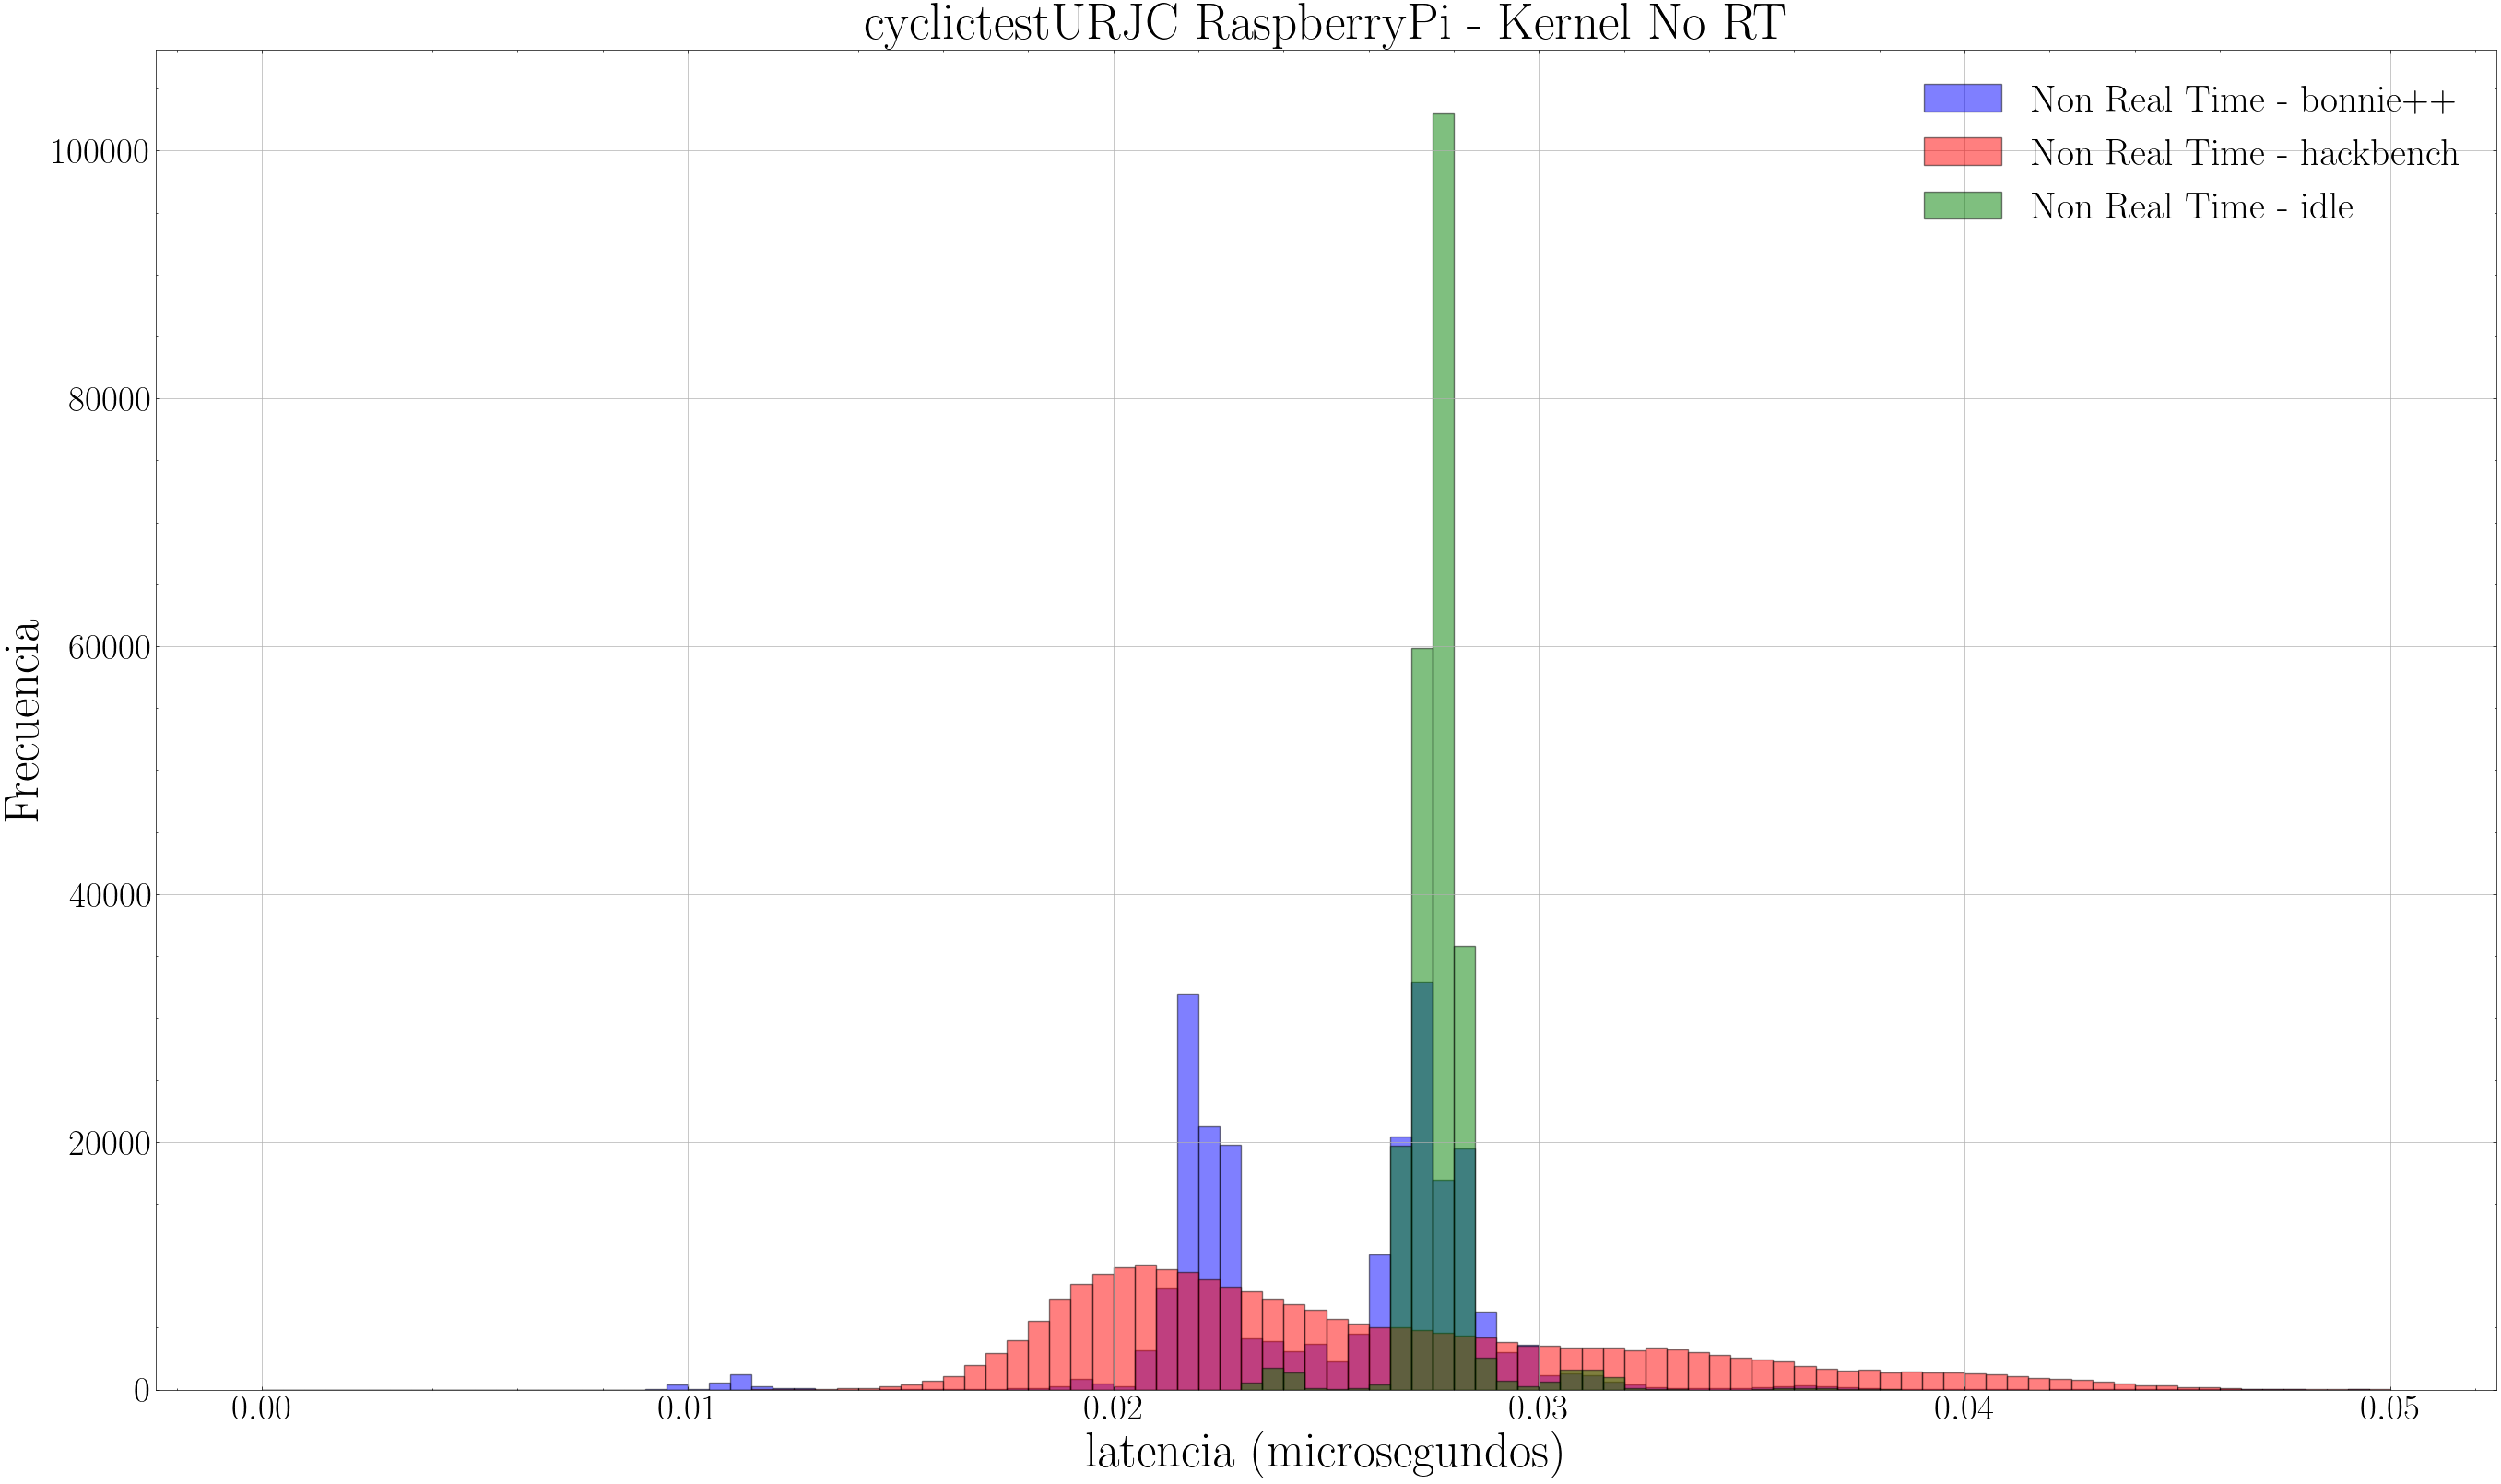
\includegraphics[width=0.7\textwidth]{noRt}
	\end{center}
	En este histograma se puede apreciar lo que he discutido en el segundo caso de la primera tabla, que usando \textit{hackbench} disminuye la latencia media, pero aumenta el rango en el que puede estar, lo que aumenta su aleatoriedad. Algo similar ocurre al usar \textit{bonnie++}. 
	\begin{center}
		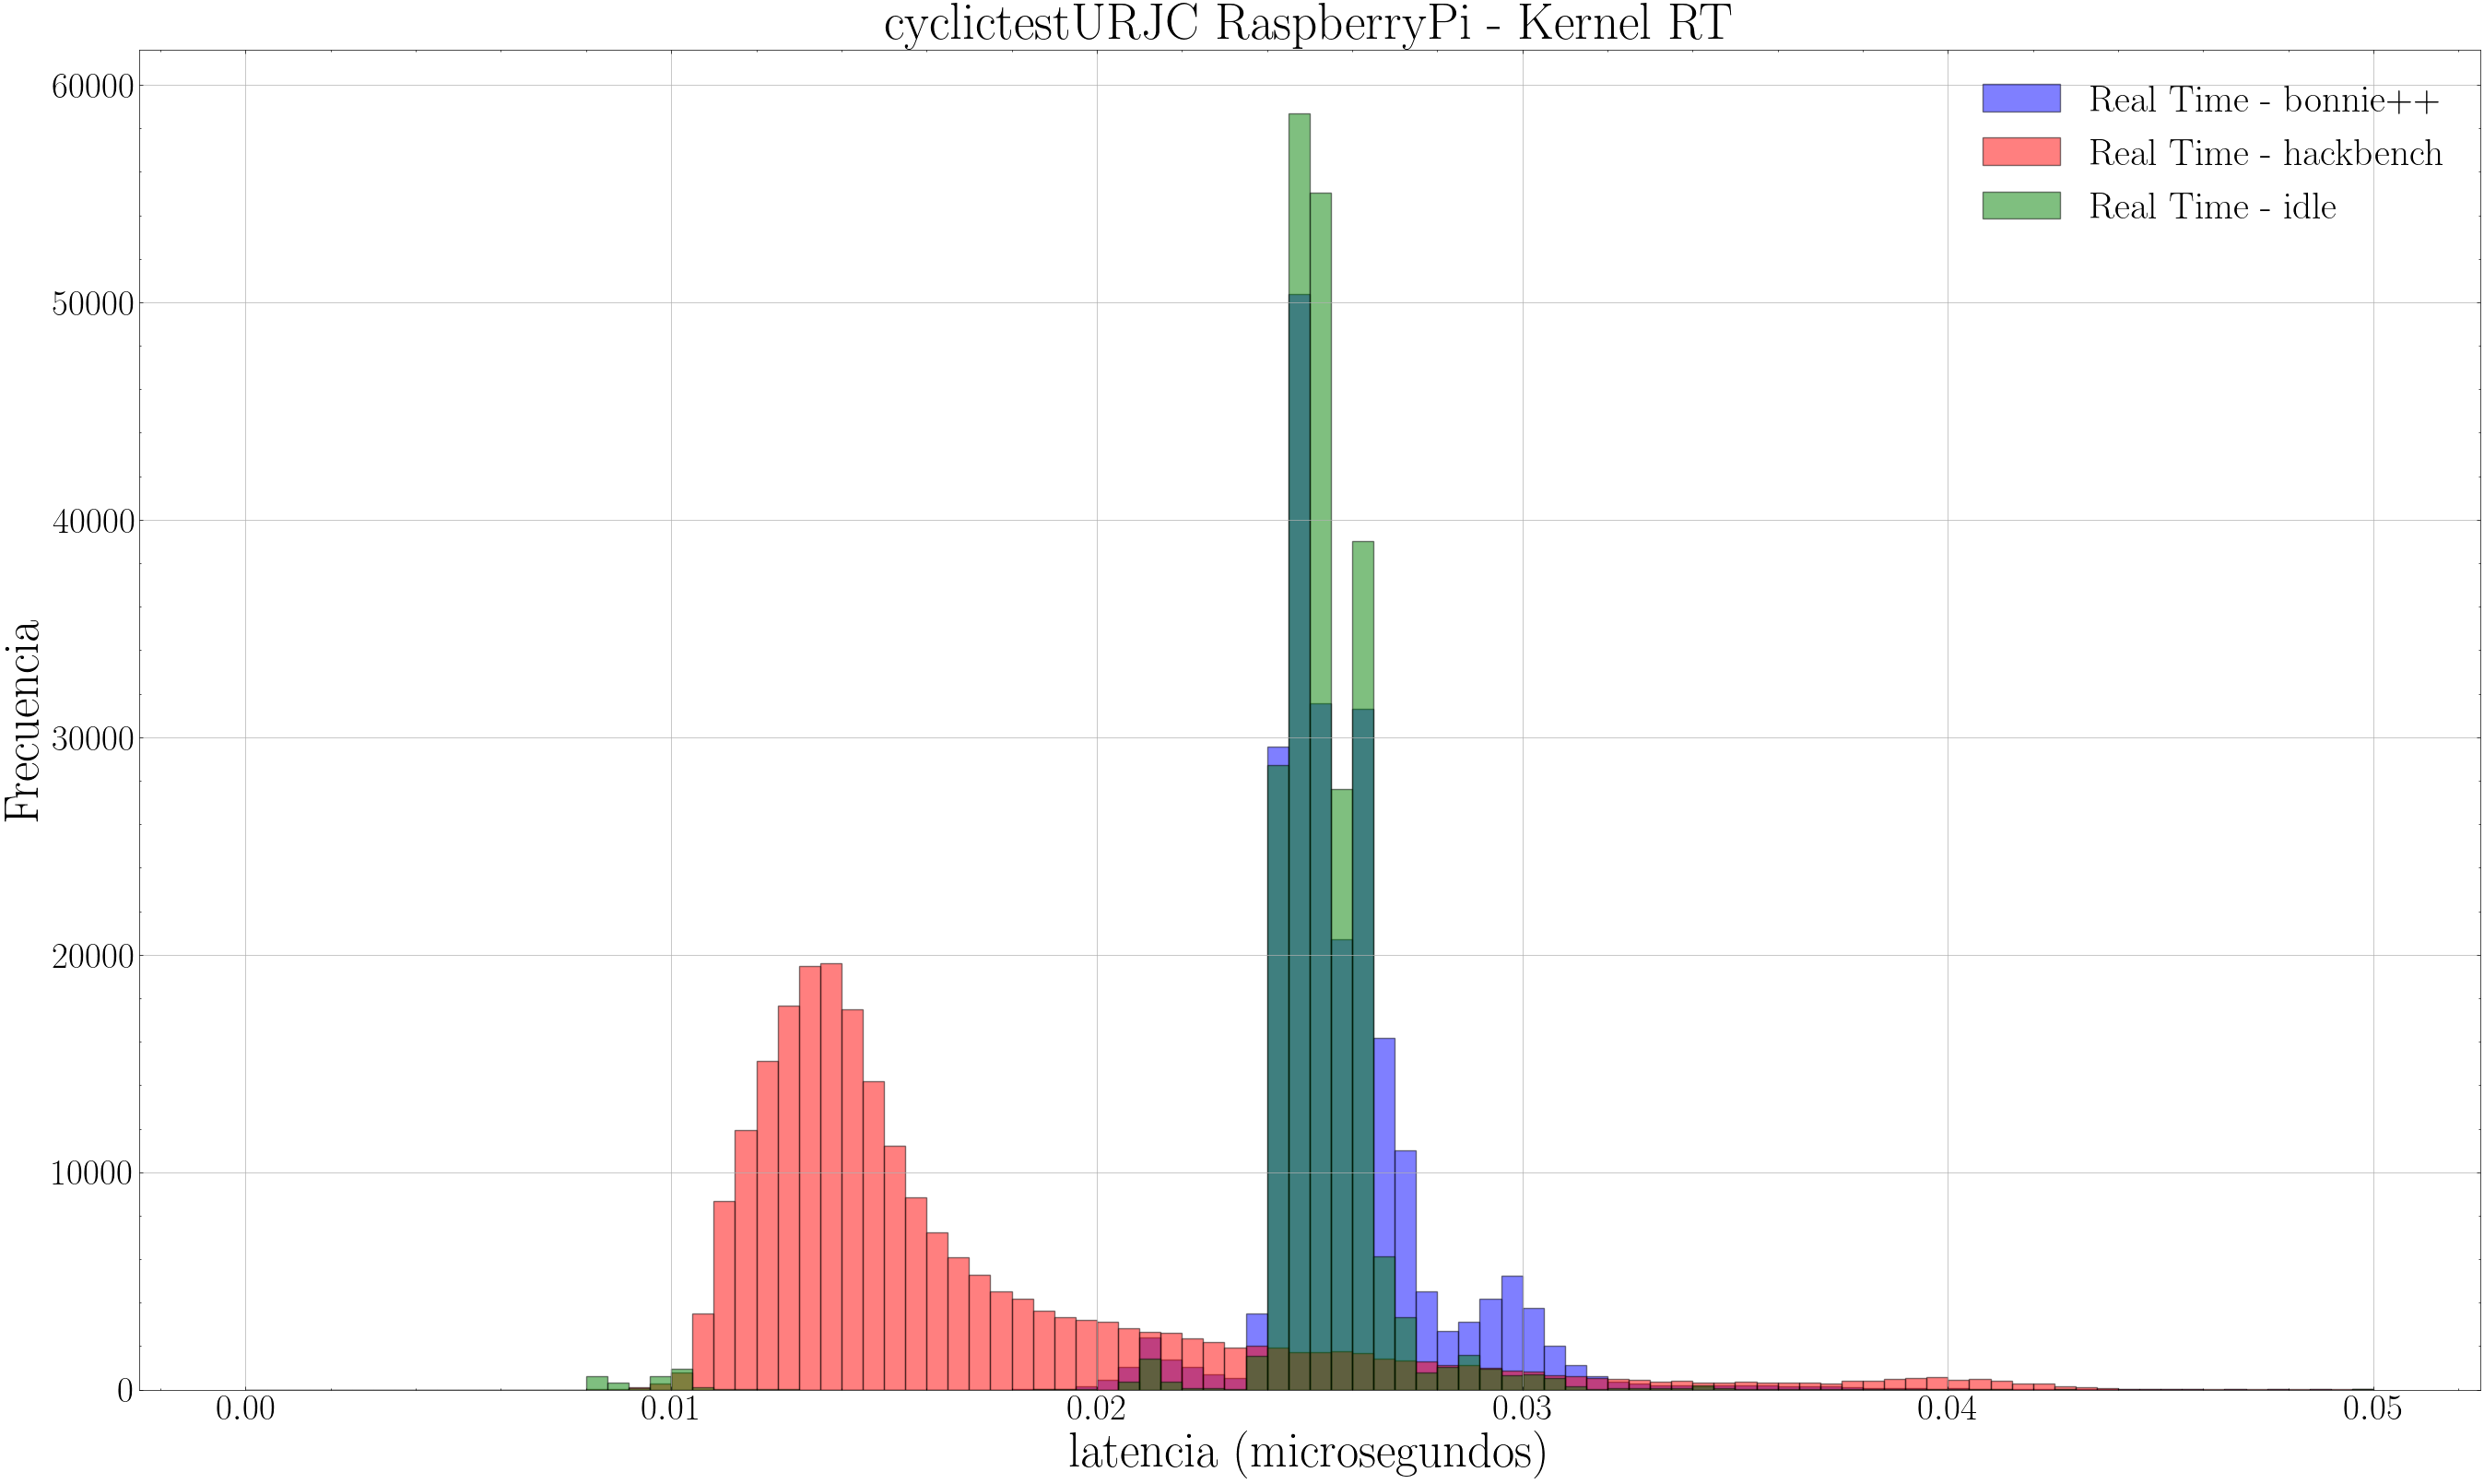
\includegraphics[width=0.7\textwidth]{Rt}
	\end{center}
\end{document}